%-------
% Gayatri Belapurkar's resume.
%-------

%-------
% Basic configurations for the document. This resume makes use of the res.cls template, a copy of which can be found 
% on https://rpi.edu/dept/arc/training/latex/resumes/ 
%-------
\documentclass[margin]{res}
\textwidth=5.2in 
            		 
% Use pdf, png, jpg, or eps§ with pdflatex; use eps in DVI mode
\usepackage{graphicx}														

\begin{document}

%---
% Defining new command for superscript usage
%---
\newcommand{\ts}{\textsuperscript} 

%----
% Basic details 
%----
\name{Gayatri Vyankatesh Belapurkar\\[13pt]}
\address{{\bf Address} \\91 A, Kamgar Nagar \\ Kurla East \\ Mumbai 400024}
\address{{\bf Contact Details} \\Mob: +91-9920697529 \\ Email: gayatri.belapurkar5@gmail.com}

\begin{resume}

%----
% Photo
%----
\begin{figure}[h!]
    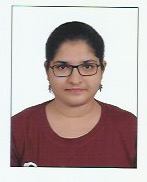
\includegraphics[scale=0.5]{Photo_gayatri.jpeg}
\end{figure}

%----
% Section: Objective
%----
\section{Objective}
Seeking a summer internship at Department of Computer Science and Engineering, IIT-Bombay under the e-Yantra Summer Internship program. 

%----
% Section: Education
%----
\section{Education}
\begin{table}[h!]
  \begin{tabular}{p{0.5cm}|p{4cm}|p{3.5cm}|p{2cm}|p{1.5cm}|p{1.6cm}}
    \textbf{Sr.} & \textbf{Degree} & \textbf{College} & \textbf{University} & \textbf{Passing Year} & \textbf{Pass Percentage} \\
    \hline
    1. & B.E., Information Technology. & Vivekanand Education Society's Institute of Technology. & University of Mumbai. & 2020 & 8.94\\
    2. & XII\ts{th} Higher Secondary Certificate. & Swami Vivekanand Junior College. & Maharashtra State Board. & 2016 & 84\%\\
    3. & X\ts{th }C.B.S.E. & Atomic Energy Central School-6. & Central Board of Secondary Education. & 2012 &  97.6\%\\
    \end{tabular}
\end{table}

%----
% Section: Projects
%----
\section{Projects}
\begin{enumerate}
  \item {\bf Smart Subsidy System using blockchain}
  
  Enter a meaningful description here. 
  \item {\bf IoT based Street Quality Identification using 'Z-algorithm' }
  
  Enter a meaningful description here. 
  \item {\bf IoT based detection of public toilet usage and incentivization}
  
  Enter a meaningful description here. 
  \item {\bf Asset Management System}
  
  Enter meaningful description here.
  \item {\bf Blockchain and web development}
  
  Enter a meaningful title and description here.
  \item {\bf App for converting text in images from English to a different language}
\end{enumerate}
  
\end{resume}

\end{document}  